\documentclass[man]{apa6}\usepackage[]{graphicx}\usepackage[]{color}
%% maxwidth is the original width if it is less than linewidth
%% otherwise use linewidth (to make sure the graphics do not exceed the margin)
\makeatletter
\def\maxwidth{ %
  \ifdim\Gin@nat@width>\linewidth
    \linewidth
  \else
    \Gin@nat@width
  \fi
}
\makeatother

\definecolor{fgcolor}{rgb}{0.345, 0.345, 0.345}
\newcommand{\hlnum}[1]{\textcolor[rgb]{0.686,0.059,0.569}{#1}}%
\newcommand{\hlstr}[1]{\textcolor[rgb]{0.192,0.494,0.8}{#1}}%
\newcommand{\hlcom}[1]{\textcolor[rgb]{0.678,0.584,0.686}{\textit{#1}}}%
\newcommand{\hlopt}[1]{\textcolor[rgb]{0,0,0}{#1}}%
\newcommand{\hlstd}[1]{\textcolor[rgb]{0.345,0.345,0.345}{#1}}%
\newcommand{\hlkwa}[1]{\textcolor[rgb]{0.161,0.373,0.58}{\textbf{#1}}}%
\newcommand{\hlkwb}[1]{\textcolor[rgb]{0.69,0.353,0.396}{#1}}%
\newcommand{\hlkwc}[1]{\textcolor[rgb]{0.333,0.667,0.333}{#1}}%
\newcommand{\hlkwd}[1]{\textcolor[rgb]{0.737,0.353,0.396}{\textbf{#1}}}%

\usepackage{framed}
\makeatletter
\newenvironment{kframe}{%
 \def\at@end@of@kframe{}%
 \ifinner\ifhmode%
  \def\at@end@of@kframe{\end{minipage}}%
  \begin{minipage}{\columnwidth}%
 \fi\fi%
 \def\FrameCommand##1{\hskip\@totalleftmargin \hskip-\fboxsep
 \colorbox{shadecolor}{##1}\hskip-\fboxsep
     % There is no \\@totalrightmargin, so:
     \hskip-\linewidth \hskip-\@totalleftmargin \hskip\columnwidth}%
 \MakeFramed {\advance\hsize-\width
   \@totalleftmargin\z@ \linewidth\hsize
   \@setminipage}}%
 {\par\unskip\endMakeFramed%
 \at@end@of@kframe}
\makeatother

\definecolor{shadecolor}{rgb}{.97, .97, .97}
\definecolor{messagecolor}{rgb}{0, 0, 0}
\definecolor{warningcolor}{rgb}{1, 0, 1}
\definecolor{errorcolor}{rgb}{1, 0, 0}
\newenvironment{knitrout}{}{} % an empty environment to be redefined in TeX

\usepackage{alltt}

\title{Always Use the Separate Variances t Test for Two Independent Groups}
\shorttitle{Separate Variances t Test}
\author{Joshua D. Wondra and Richard Gonzalez}
\affiliation{University of Michigan}

\abstract{This is an abstract}
\keywords{t test, new statistics}
\IfFileExists{upquote.sty}{\usepackage{upquote}}{}
\begin{document}
\maketitle

This is an introduction

\section{Method}

\section{Results}



We report the observed Type I error rates, observed power, and coverage probability for the classic and separate variance t tests.

\subsection{Type I Error Rates}
In this section we report type I error rates for the classic and separate variance t tests when the null hypothesis is true. Prior research has demonstrated that when either sample sizes or variances are equal, the type I error rates are preserved at .05 for both tests (CITATIONS). 

\subsubsection{Equal Variances, Different Sample Sizes}
Consistent with prior research, the type I error rate was .05 for both the classic and separate variance t tests across all sample sizes and sample size ratio.

\subsubsection{Equal Sample Sizes, Different Variances}
Consistent with prior research, the type I error rate was .05 for both the classic and separate variance t tests across all sample sizes and variance ratios.

\subsubsection{Different Sample Sizes, Different Variances}
Consistent with prior research, the classic t test was not robust when both variances and sample sizes were equal. When the group with the bigger sample also had the bigger variance, the classic t test was more conservative; the type I error rate dropped as low as .01 when the large group had twice the sample size and five times the variance of the small group (see Figure 1). When the group with the bigger sample had the smaller variance, however, the classic t test was more liberal; the type I error rate inflated to just over .12 when the large group had twice the sample size and five times the variance of the small group (see Figure 2). In all cases, however, the separate variances t test approximately  maintained the expected type I error rate of .05.

\begin{knitrout}
\definecolor{shadecolor}{rgb}{0.969, 0.969, 0.969}\color{fgcolor}
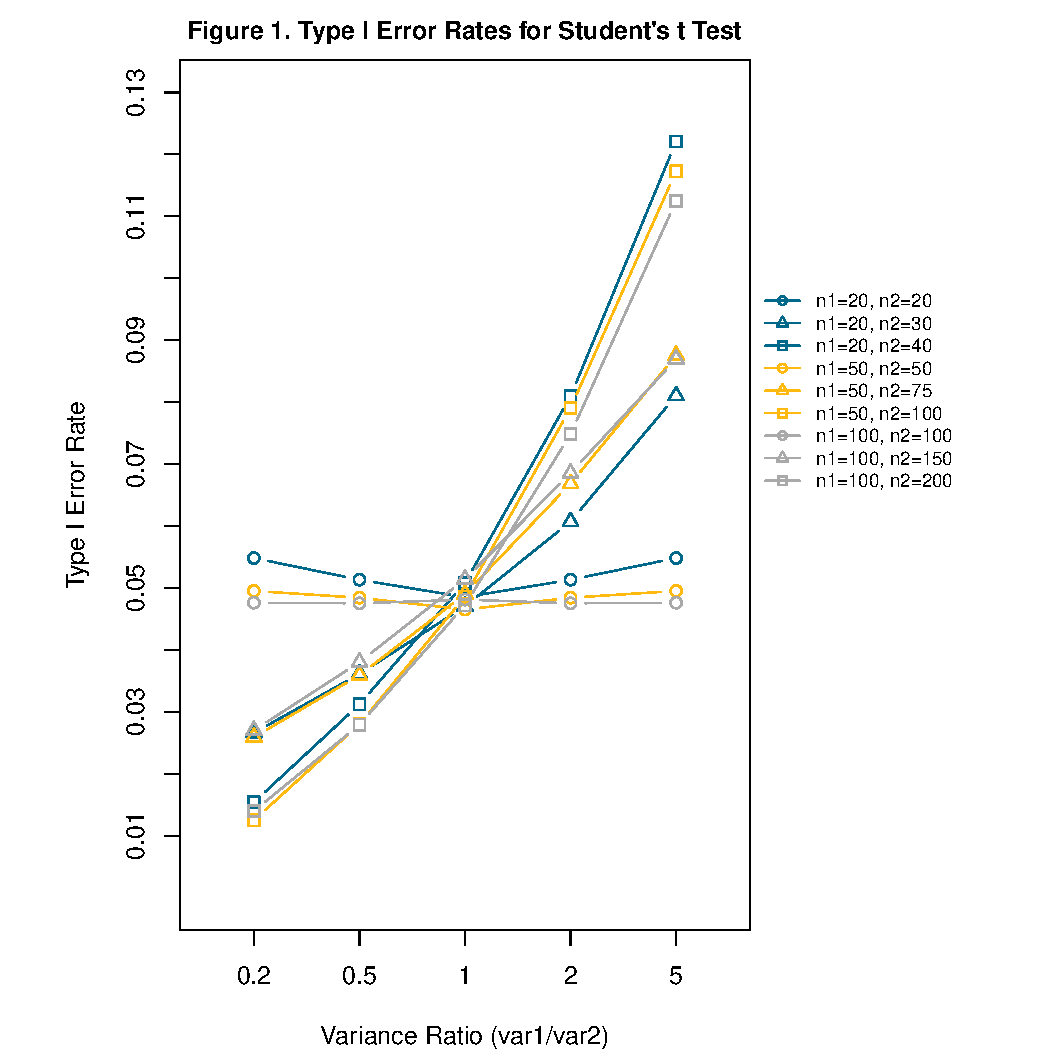
\includegraphics[width=\maxwidth]{figure/ssv_type11} 

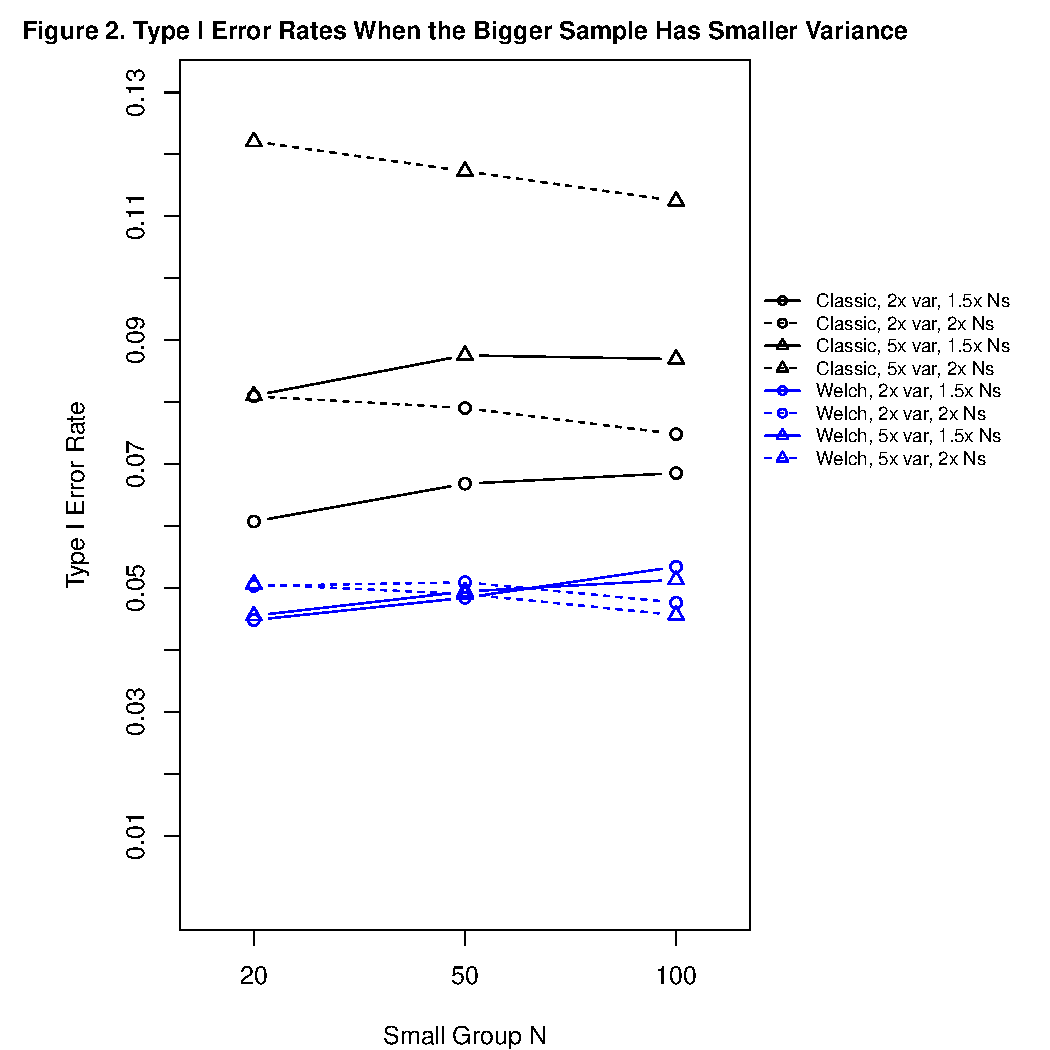
\includegraphics[width=\maxwidth]{figure/ssv_type12} 

\end{knitrout}



\subsection{Power}

\subsection{Coverage Probability}


\end{document}
